%%%%%%%%%%%%%%%%%%%%%%%%%%%%%%%%%%%%%%%%%%%%%%%%%%%%%%%%%%%%%%%%
%%                                                            %%
%%   essentialsOfLatin, Italian translation 2017              %%
%%                                                            %%
%% From:  Henry C. Pearson, Essentials Of Latin For Beginners %%
%%        (1915, New York, American Book Company)             %%
%%                                                            %%
%%    https://archive.org/details/essentialslatin04peargoog   %%
%%                                                            %%
%% Translated by g.p.ciceri <gp.ciceri@gmail.com>             %%
%% ---------------------------------------------------------- %%
%% This translation is Licensed under                         %%
%% Creative Commons Attribution-ShareAlike 4.0 International  %%
%% https://creativecommons.org/licenses/by-sa/4.0/            %%
%%                                                            %%
%%%%%%%%%%%%%%%%%%%%%%%%%%%%%%%%%%%%%%%%%%%%%%%%%%%%%%%%%%%%%%%%

% āēīōū
% ăĕĭŏŭ




\documentclass[nols]{tufte-handout}

%\geometry{showframe} % display margins for debugging page layout

\usepackage{fontspec}
\usepackage{ifxetex}
\setmainfont[Path=./fonts/palatino-linotype/, ItalicFont=palai.ttf, BoldFont=palab.ttf]{pala.ttf}


% \defaultfontfeatures{Mapping=tex-text}
% \setromanfont[Path=./fonts/TeX-Gyre-Schola/,Mapping=tex-text]{TeX Gyre Schola}
% \setsansfont[Path=./fonts/TeX-Gyre-Heros/,Scale=MatchLowercase,Mapping=tex-text]{TeX Gyre Heros}
% \setmonofont[Path=./fonts/TeX-Gyre-Cursor/,Scale=MatchLowercase]{TeX Gyre Cursor}

\usepackage{lipsum}
\usepackage{url}
\usepackage{longtable}
\usepackage{stackengine}

\usepackage{graphicx} % allow embedded images
  \setkeys{Gin}{width=\linewidth,totalheight=\textheight,keepaspectratio}
  \graphicspath{{graphics/}} % set of paths to search for images
\usepackage{amsmath}  % extended mathematics
\usepackage{booktabs} % book-quality tables
\usepackage{units}    % non-stacked fractions and better unit spacing
\usepackage{multicol} % multiple column layout facilities
\usepackage{lipsum}   % filler text
\usepackage{fancyvrb} % extended verbatim environments
  \fvset{fontsize=\normalsize}% default font size for fancy-verbatim environments

% Standardize command font styles and environments
\newcommand{\doccmd}[1]{\texttt{\textbackslash#1}}% command name -- adds backslash automatically
\newcommand{\docopt}[1]{\ensuremath{\langle}\textrm{\textit{#1}}\ensuremath{\rangle}}% optional command argument
\newcommand{\docarg}[1]{\textrm{\textit{#1}}}% (required) command argument
\newcommand{\docenv}[1]{\textsf{#1}}% environment name
\newcommand{\docpkg}[1]{\texttt{#1}}% package name
\newcommand{\doccls}[1]{\texttt{#1}}% document class name
\newcommand{\docclsopt}[1]{\texttt{#1}}% document class option name
\newenvironment{docspec}{\begin{quote}\noindent}{\end{quote}}% command specification environment

% concetti morfosintattici
\usepackage{xspace} 
\newcommand{\noun}{\textsc{sostantivo}\xspace}
\newcommand{\nouns}{\textsc{sostantivi}\xspace}
\newcommand{\adject}{\textsc{aggettivo}\xspace}
\newcommand{\adjects}{\textsc{aggettivi}\xspace}
\newcommand{\gnumber}{\textsc{numero}\xspace}
\newcommand{\gnumbers}{\textsc{numeri}\xspace}
\newcommand{\gender}{\textsc{genere}\xspace}
\newcommand{\genders}{\textsc{generi}\xspace}
\newcommand{\gcase}{\textsc{caso}\xspace}
\newcommand{\gcases}{\textsc{casi}\xspace}
\newcommand{\tense}{\textsc{tempo}\xspace}
\newcommand{\mood}{\textsc{modo}\xspace}
\newcommand{\gverb}{\textsc{verbo}\xspace}
\newcommand{\gverbs}{\textsc{verbi}\xspace}
\newcommand{\adjective}{\textsc{aggettivo}\xspace}
\newcommand{\nom}{\textsc{nom}\xspace}
\newcommand{\gen}{\textsc{gen}\xspace}
\newcommand{\dat}{\textsc{dat}\xspace}
\newcommand{\acc}{\textsc{acc}\xspace}
\newcommand{\voc}{\textsc{voc}\xspace}
\newcommand{\abl}{\textsc{abl}\xspace}
\newcommand{\gexit}{\textsc{uscita}\xspace}
\newcommand{\gexits}{\textsc{uscite}\xspace}
\newcommand{\declinazione}{\textsc{declinazione}\xspace}
\newcommand{\masc}{\textsc{maschile}\xspace}
\newcommand{\femm}{\textsc{femminile}\xspace}
\newcommand{\neut}{\textsc{neutro}\xspace}

\newcommand{\indic}{\textsc{indicativo}\xspace}
\newcommand{\imper}{\textsc{imperativo}\xspace}
\newcommand{\gcong}{\textsc{congiuntivo}\xspace}
\newcommand{\ott}{\textsc{ottativo}\xspace}
\newcommand{\partic}{\textsc{participio}\xspace}
\newcommand{\infin}{\textsc{infinito}\xspace}

\newcommand{\pres}{\textsc{presente}\xspace}
\newcommand{\imperf}{\textsc{imperfetto}\xspace}
\newcommand{\aor}{\textsc{aoristo}\xspace}
\newcommand{\fut}{\textsc{futuro}\xspace}
\newcommand{\perf}{\textsc{perfetto}\xspace}
\newcommand{\pperf}{\textsc{piuccheperfetto}\xspace}

\newcommand{\sing}{\textsc{singolare}\xspace}
\newcommand{\plur}{\textsc{plurale}\xspace}
\newcommand{\dual}{\textsc{duale}\xspace}

\newcommand{\si}{\textsc{sing}\xspace}
\newcommand{\pl}{\textsc{plur}\xspace}
\newcommand{\du}{\textsc{dual}\xspace}

\newcommand{\att}{\textsc{attivo}\xspace}
\newcommand{\med}{\textsc{medio}\xspace}
\newcommand{\pass}{\textsc{passivo}\xspace}
\newcommand{\medpass}{\textsc{medio-passivo}\xspace}


% italianitudini
\renewcommand{\figurename}{Figura}
\renewcommand{\tablename}{Tabella}
\renewcommand{\contentsname}{Indice}

% fix per un qualche problema
\ifxetex
  \newcommand{\textls}[2][5]{%
    \begingroup\addfontfeatures{LetterSpace=#1}#2\endgroup
  }
  \renewcommand{\allcapsspacing}[1]{\textls[15]{#1}}
  \renewcommand{\smallcapsspacing}[1]{\textls[10]{#1}}
  \renewcommand{\allcaps}[1]{\textls[15]{\MakeTextUppercase{#1}}}
  \renewcommand{\smallcaps}[1]{\smallcapsspacing{\scshape\MakeTextLowercase{#1}}}
  \renewcommand{\textsc}[1]{\smallcapsspacing{\textsmallcaps{#1}}}
\fi

% too many float...
\extrafloats{100}
% āēīōū
% ăĕĭŏŭ

\title{Essentials Of Latin. Elementi di Latino. \newline Lezione X - Imperfetto e Futuro di sum. Ripasso}

\author[gpciceri]{a cura di Milagathòs: Milo's help to enjoy humanities.}

\date{23 Febbrajo 2017} % without \date command, current date is supplied


\begin{document}

\hyphenation{co-niu-ga-zio-ne}

\maketitle% this prints the handout title, author, and date

\begin{marginfigure}[-2.5cm]
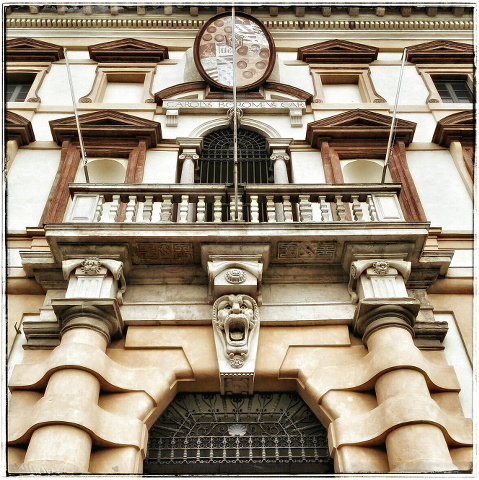
\includegraphics{smallthumb-lesson_I.jpeg}
\setfloatalignment{b}
\end{marginfigure}


\begin{abstract}
\noindent
Queste lezioni riprendono il testo introduttivo al Latino di Pearson\cite{pearson1915}, del quale seguono la numerazione; la struttura di ogni lezione è piuttosto regolare: inizia con \textsc{cenni di morfologia e di sintassi latina}, seguita da un \textsc{piccolo vocabolario} per il lessico; ci sono infine vari \textsc{esercizi} di traduzione e di composizione latina.

\bigskip
\noindent
Lezione X - Imperfetto e futuro di sum. Ripasso, vocaboli, esercizi, lettura.
\end{abstract}

%\printclassoptions

% āēīōū
% ăĕĭŏŭ

\newthought{81. Ripassa il (39.).} L'imperfetto e il futuro indicativo di \textbf{sum} sono coniugati in questo modo: 

\begin{fullwidth}
\begin{table}[!htbp]
  \centering
  \begin{tabular}{l l l l l}
    %\toprule
	& \multicolumn{1}{c}{\textsc{Imperfetto}} & \hspace{20mm} & & \multicolumn{1}{c}{\textsc{Future}} \\
	\multicolumn{5}{c}{\textsc{Singolare}} \\

    \textsc{1.} & era\textbf{m}, \textit{io ero}   & \hspace{20mm} & \textsc{1.} & er\textbf{ō}, \textit{io sarò}    \\
    \textsc{2.} & erā\textbf{s}, \textit{tu eri}   & \hspace{20mm} & \textsc{2.} & eri\textbf{s}, \textit{tu sarai}    \\
    \textsc{3.} & era\textbf{t}, \textit{egli era, c'era} & \hspace{20mm} & \textsc{3.} & eri\textbf{t}, \textit{egli sarà, ci sarà}    \\
   
	\multicolumn{5}{c}{\textemdash} \\
	
    \multicolumn{5}{c}{\textsc{Plurale}} \\

    \textsc{1.} & erā\textbf{mus}, \textit{noi eravamo}        & \hspace{20mm} & \textsc{1.} & eri\textbf{mus}, \textit{noi saremo}    \\
    \textsc{2.} & erā\textbf{tis}, \textit{voi eravate}        & \hspace{20mm} & \textsc{2.} & eri\textbf{tis}, \textit{voi sarete}    \\
    \textsc{3.} & era\textbf{nt}, \textit{essi erano, c'erano} & \hspace{20mm} & \textsc{3.} & eru\textbf{nt}, \textit{essi saranno, ci saranno}    \\

    %\bottomrule
  \end{tabular}
  %\caption[bottom]{Prima Declinazione. \textbf{stella, -ae}, f.}
  \label{tab:normaltab}
  %\zsavepos{pos:normaltab}
\end{table}
\end{fullwidth}

\begin{itemize}
\item[\textsc{1.}] Le terminazioni personali sono regolari (cfr. (43.))? Sono uguali a quelle del presente di \textbf{sum}?  
\end{itemize}


\newthought{82. Ordine delle Parole.} In una frase in italiano (come in inglese), l'ordine delle parole è importante, 
dal momento che ci sono poche flessioni (rispetto al latino). Cambiare l'ordine delle parole può voler dire cambiar senso alla frase.
Ad Esempio:
\\
\textit{Cesare loda i contadini leali} \\
\textit{I contadini leali lodano Cesare} \\
In latino, cambiare l'ordine delle parole non cambia - solitamente - il significato della frase, ma indica solo textit{l'enfasi} che l'autore
ha voluto dare a una parola particolare. Ad esempio:
\begin{itemize}
\item[\textsc{1.}] \textbf{Caesar agricolas fidos laudat}, \textit{Cesare loda i contadini leali}.  
\item[\textsc{1.}] \textbf{Caesar fidos agricolas laudat}, \textit{Cesare loda i contadini leali}.  
\item[\textsc{1.}] \textbf{Agricolas fidos laudat Caesar}, \textit{Cesare loda i contadini leali}.  
\end{itemize}
La prima frase mostra l'ordine normale \sidenote{ordine normale di una frase latina: (i) soggetto con i suoi modificatori, 
(ii) oggetto indiretto con i suoi modificatori,
(iii) oggetto diretto con i suoi modificatori,
(iv) avverbi, (v) verbo.} e non mette enfasi su alcuna parola. Questo ordine è spesso variato dall'autore per esprimere enfasi: 
nella seconda frase l'aggettivo \textbf{fidos} è più enfatico rispetto alla prima, nella terza sia \textbf{agricolas fidos} che \textbf{Caesar} sono enfatici.

\newthought{83. Ripasso dei nomi della Prima e Seconda Declinazione.}
\begin{itemize}
\item[\textsc{1.}] Ripassa con attenzione significato, genere e declinazione di ogni nome.  
\item[\textsc{2.}] Ricollega ogni parola latina con i suoi derivati italiani (ad es.: \textbf{vita}, \textit{vitale}; \textbf{nauta}, \textit{nautico}) e raggruppa le parole latine per tema (ad es.: \textbf{ager}, \textit{campo}; \textbf{agricola}, \textit{contadino}). \textit{Fai questo per le parole nuove nei vocabolari che seguiranno}. 
\end{itemize}

\begin{multicols}{5}
incola \\
discipulus \\
vīnum \\
sagitta \\
proelium \\
puer \\ 
via \\ 
rosa \\
cibus \\ 

gladius \\ 
vir \\
ager \\
fēmina \\
nuntius \\
hortus \\
silva \\
inopia \\
nauta \\ 

agricola \\ 
patria \\
cōpia \\ 
vita \\
pecunia \\
terra  \\
rēgīna  \\
stella  \\
equus  \\

lūna  \\
porta  \\
fabula \\
insula \\
amīcus  \\
dominus  \\
servus  \\
fīlia  \\
fīlius  \\

aedificium \\ 
frūmentum  \\
oppidum \\
dōnum  \\
bellum  \\
magister  \\
liber 

\end{multicols}



\newthought{80. Esercizi}
\\
\textsc{I.} \quad
\textsc{1.}~Erimus; eramus; sumus. \quad
\textsc{2.}~Eratis; eritis; estis. \quad
\textsc{3.}~Erant; es; eris. \quad
\textsc{4.}~Eras; erunt; eris. \quad
\textsc{5.}~Fllii agricolae erant parvi. \quad
\textsc{6.}~Filia nuntl erat in insula pulchra. \quad
\textsc{7.}~Reginae copiae erunt in tua patria. \quad
\textsc{8.}~Nautae non erant pigri. \quad
\textsc{9.}~Ubi gladius mei amici erat? \quad
\textsc{10.}In magno aedificio erat.
\\
\textsc{II.} \quad
\textsc{1.}~Noi eravamo; noi siamo; noi saremo. \quad
\textsc{2.}~Essi saranno; voi sarete; ella era. \quad
\textsc{3.}~Tu eri; egli sarà; tu sarai. \quad
\textsc{4.}~Il cavallo del mio amico non era pigro. \quad
\textsc{5.}~I figli del marinaio erano piccoli. \quad
\textsc{6.}~I fieri abitanti saranno schiavi della regina.

\newthought{(443.) Lettura e Traduzione.} Bambini romani.
\\
Europae terra Italia est. Roma magnum in Italia oppidum est.
Multae portae, bonae et latae viae, alba aedificia in oppido sunt.
Horti incolarum superborum magni sunt. In hortis Marci ludus est.
Magister, vir, peritus, liberos convocat. Equi validi parvos liberos
in hortos magistri portant. Cur mali pueri pugnant? Asperi sunt.
Pueri amant bella et proelia et sagittas et gladios.
Puellas teneras rosae albae in hortis, nova luna, parvae stellae delectant.
Magister malos et pigros discipulos culpat, sed bonos (discipulos) amat.
Pulchros libros dona bonis pueris et puellis dat. In libris multae fabulae Romam oppidum laudant.



\begin{figure}[!b]
  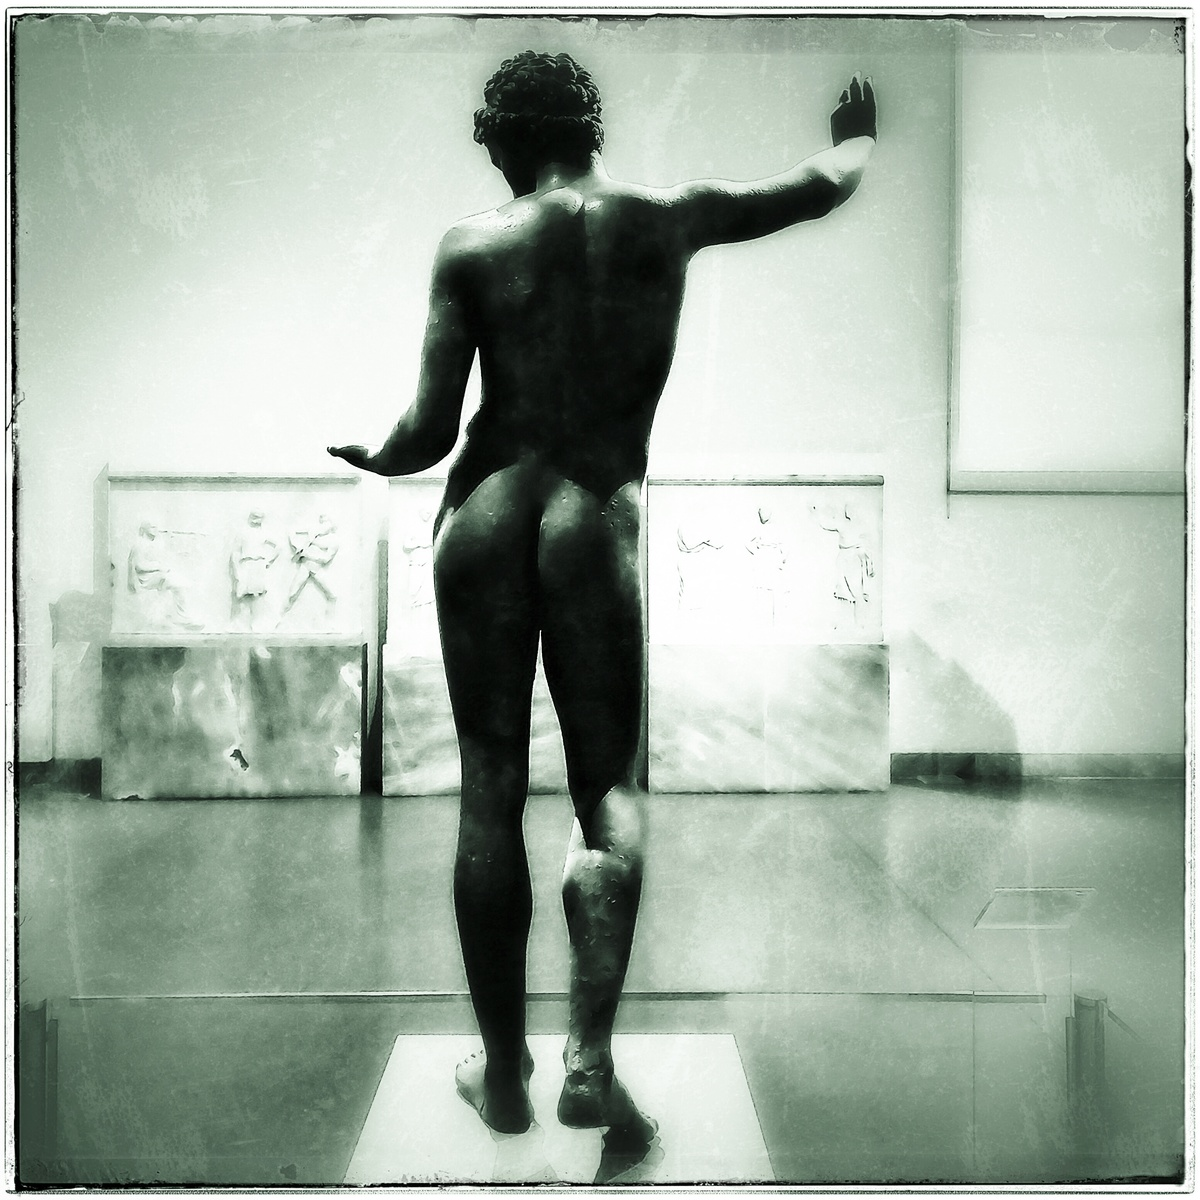
\includegraphics[width=0.8\linewidth]{thumb-lesson_VII.jpeg}
  %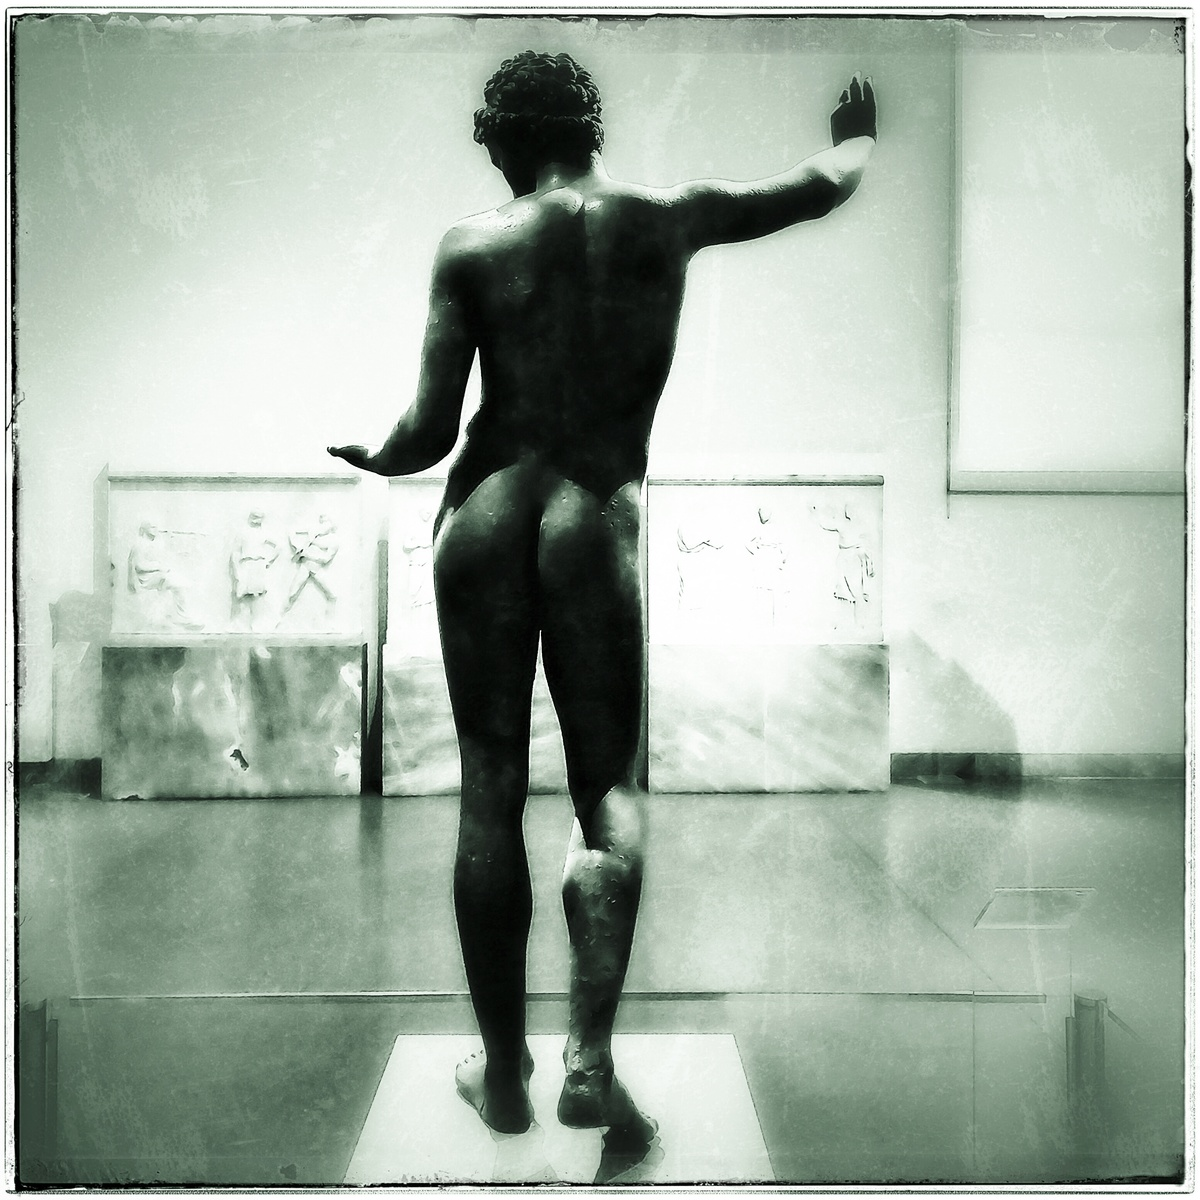
\includegraphics{thumb-lesson_VII.jpeg}
  \caption{Pavia: Almo Collegio Borromeo}
  \label{fig:textfig}
  %\zsavepos{pos:textfig}
  %\setfloatalignment{b}
\end{figure}

 

\nobibliography{latinBiblio}
\bibliographystyle{alpha}


\end{document}
